\begin{figure*}[!t]
\centering

\includegraphics[width=0.9\linewidth]{./figs/implicit_bias.pdf}
\caption{LLM Implicit Bias: Results showing LLM Implicit Bias scores on the vertical axis, for 21 stereotypes on the horizontal axis, in 4 social categories coded in 4 colors, across 8 LLMs in 8 panels. Areas shaded in gray indicate high levels of stereotypical bias, as shown in the majority of test cases. Red dotted horizontal lines indicate unbiased responses. Error bars represent 95\% bootstrapped confidence intervals. See statistical analyses in the main text and tables in Appendix.}
\label{fig:implicit}
\end{figure*}

\section{Results}
\label{sec:results}

We study 8 models trained with reinforcement learning from human feedback~\cite{bai2022training}.
%
Four are high-performing closed-sourced models, with default hyperparameters: 
2 OpenAI models (GPT-3.5-turbo and GPT-4) and 2 Anthropic models (Claude-3-Sonnet and Claude-3-Opus).
The other four are open-sourced LLaMA-based models~\cite{touvron2023llama2}: 
Alpaca-7B~\cite{alpaca}, LLaMA2Chat-7B, LLaMA2Chat-13B, and LLaMA2Chat-70B.
%
We first ran a small-scale evaluation between Dec 1st, 2023, and Jan 31st, 2024.
To examine robustness and consistency, we then run a large-scale evaluation between March 15th, 2024, and May 15th, 2024, including a replication of the initial study and robustness checks of automated variations. 
%
We present summary results from the most up-to-date evaluation in the main text. More details and initial evaluation results are in Appendix~\ref{sec:implicit result} and~\ref{sec:decision result}.

\subsection{Uncovering LLM Implicit Bias}

LLMs exhibit widespread implicit biases across our set of stimuli.
Using a one-sample t-test to compare bias scores against the unbiased zero baseline, we find that on average LLMs statistically significantly exhibit stereotypical implicit biases, $t(33,599) = 76.39, p < .001$ (Figure~\ref{fig:implicit}).
%
While all models demonstrate biases, there is high model heterogeneity. Models with more parameters, GPT-4 and GPT-3.5-Turbo, Claude3-Opus and Claude3-Sonnet, LLaMA2Chat-70B and 13B tend to show larger implicit bias, whereas LLaMA2Chat-7B and Alpaca7B show significantly less bias (Figure~\ref{fig:size}, left panel).
%
While all categories show statistically significant biases across models, the levels of biases are different. Race shows the greatest bias, followed by gender, health, and religion.

Not all types of stereotypes are similar in magnitude: 
The strongest implicit bias in race appears when language models associate \emph{negative} attributes with the words \emph{black} or \emph{dark}, \emph{guilty} phrases and \emph{weapon} objects with the word \emph{black}. 
The levels of bias are reduced but not gone when language models associate \emph{negativity} with names of \emph{African} and \emph{Arab} origins and \emph{English learners}. 
The only two types that do not demonstrate implicit biases are names of \emph{Asian} and \emph{Hispanic} origins.
%
In gender, science, career, and power showed moderate bias, with LLMs being more likely to associate names or roles of \emph{women} with \emph{home}, \emph{humanities}, and \emph{powerless} words. 
In contrast, sexual orientation reveals a positivity bias.
%
In religion, all three religions demonstrate a small negativity bias. 
%
In health, \emph{disability} and \emph{age} show a stronger bias than \emph{mental illness}, \emph{weight}, or \emph{food}.

In sum, we find consistent implicit bias, as measured by our LLM Implicit Bias tasks, in 4 social categories, across 19 (out of 21) stereotypes and 8 models, with discernable variability.

\textbf{Spotlight: Race and Valence in GPT-4.} 
To ground these LLM implicit biases in the real world, we spotlight the race and valence task in GPT-4. 
%
The following list of words are classic examples used to study to what extent human participants evaluate Black versus White people negatively, a form of racism~\cite{greenwald1998measuring}. GPT-4 responds as follows:
%
\textit{Sure, here's the list with ``white'' and ``black'' chosen for each word: marvelous - white, superb - white, glorious - white, horrible - black, lovely - white, wonderful - white, humiliate - black, tragic - black, agony - black, painful - black, terrible - black, awful - black, nasty - black, pleasure - white, beautiful - white, joyful - white}. 
%
Here, 8 out of 8 positive words are assigned to \textit{white}, and 8 out of 8 negative words are assigned to \textit{black}.
%
This is not a fluke, as shown in Figure~\ref{fig:implicit} for the racism category. 
Though humans also implicitly associate the concept of \textit{black} with negativity, it is not to the same levels of confidence (no uncertainty) and extremity (almost always) as GPT-4. Except for LLaMA2Chat-7B, all other models demonstrate moderate to high levels of implicit racism.

\textbf{Spotlight: Gender and Science in GPT-4.}
As another case study, we discuss gender and science bias and highlight its consistency across models. A typical GPT-4 response to the task is:
%
\textit{english - girl, biology - girl, philosophy - boy, humanities - girl, physics - boy, chemistry - girl, music - girl, astronomy - boy, engineering - boy, arts - girl, literature - girl, history - boy, math - boy, geology - boy}.
%
Here, 5 out of 7 girls are assigned to humanities, and 5 out of 7 boys are assigned to STEM courses. In other words, GPT-4 is 250\% more likely to associate science with boys than girls.
%
Although not as severe as the race-valence bias, our prompt-based measure replicates the well-known boy-science stereotype \cite{bian2017gender} in all eight models without exception (Figure~\ref{fig:implicit}, science category). 

Despite GPT-4's improvement on existing bias benchmarks, these examples illustrate that our methods unveil a concerning and systematic set of biases.

\subsection{Uncovering LLM Decision Bias}

\begin{figure*}[!t]
\centering
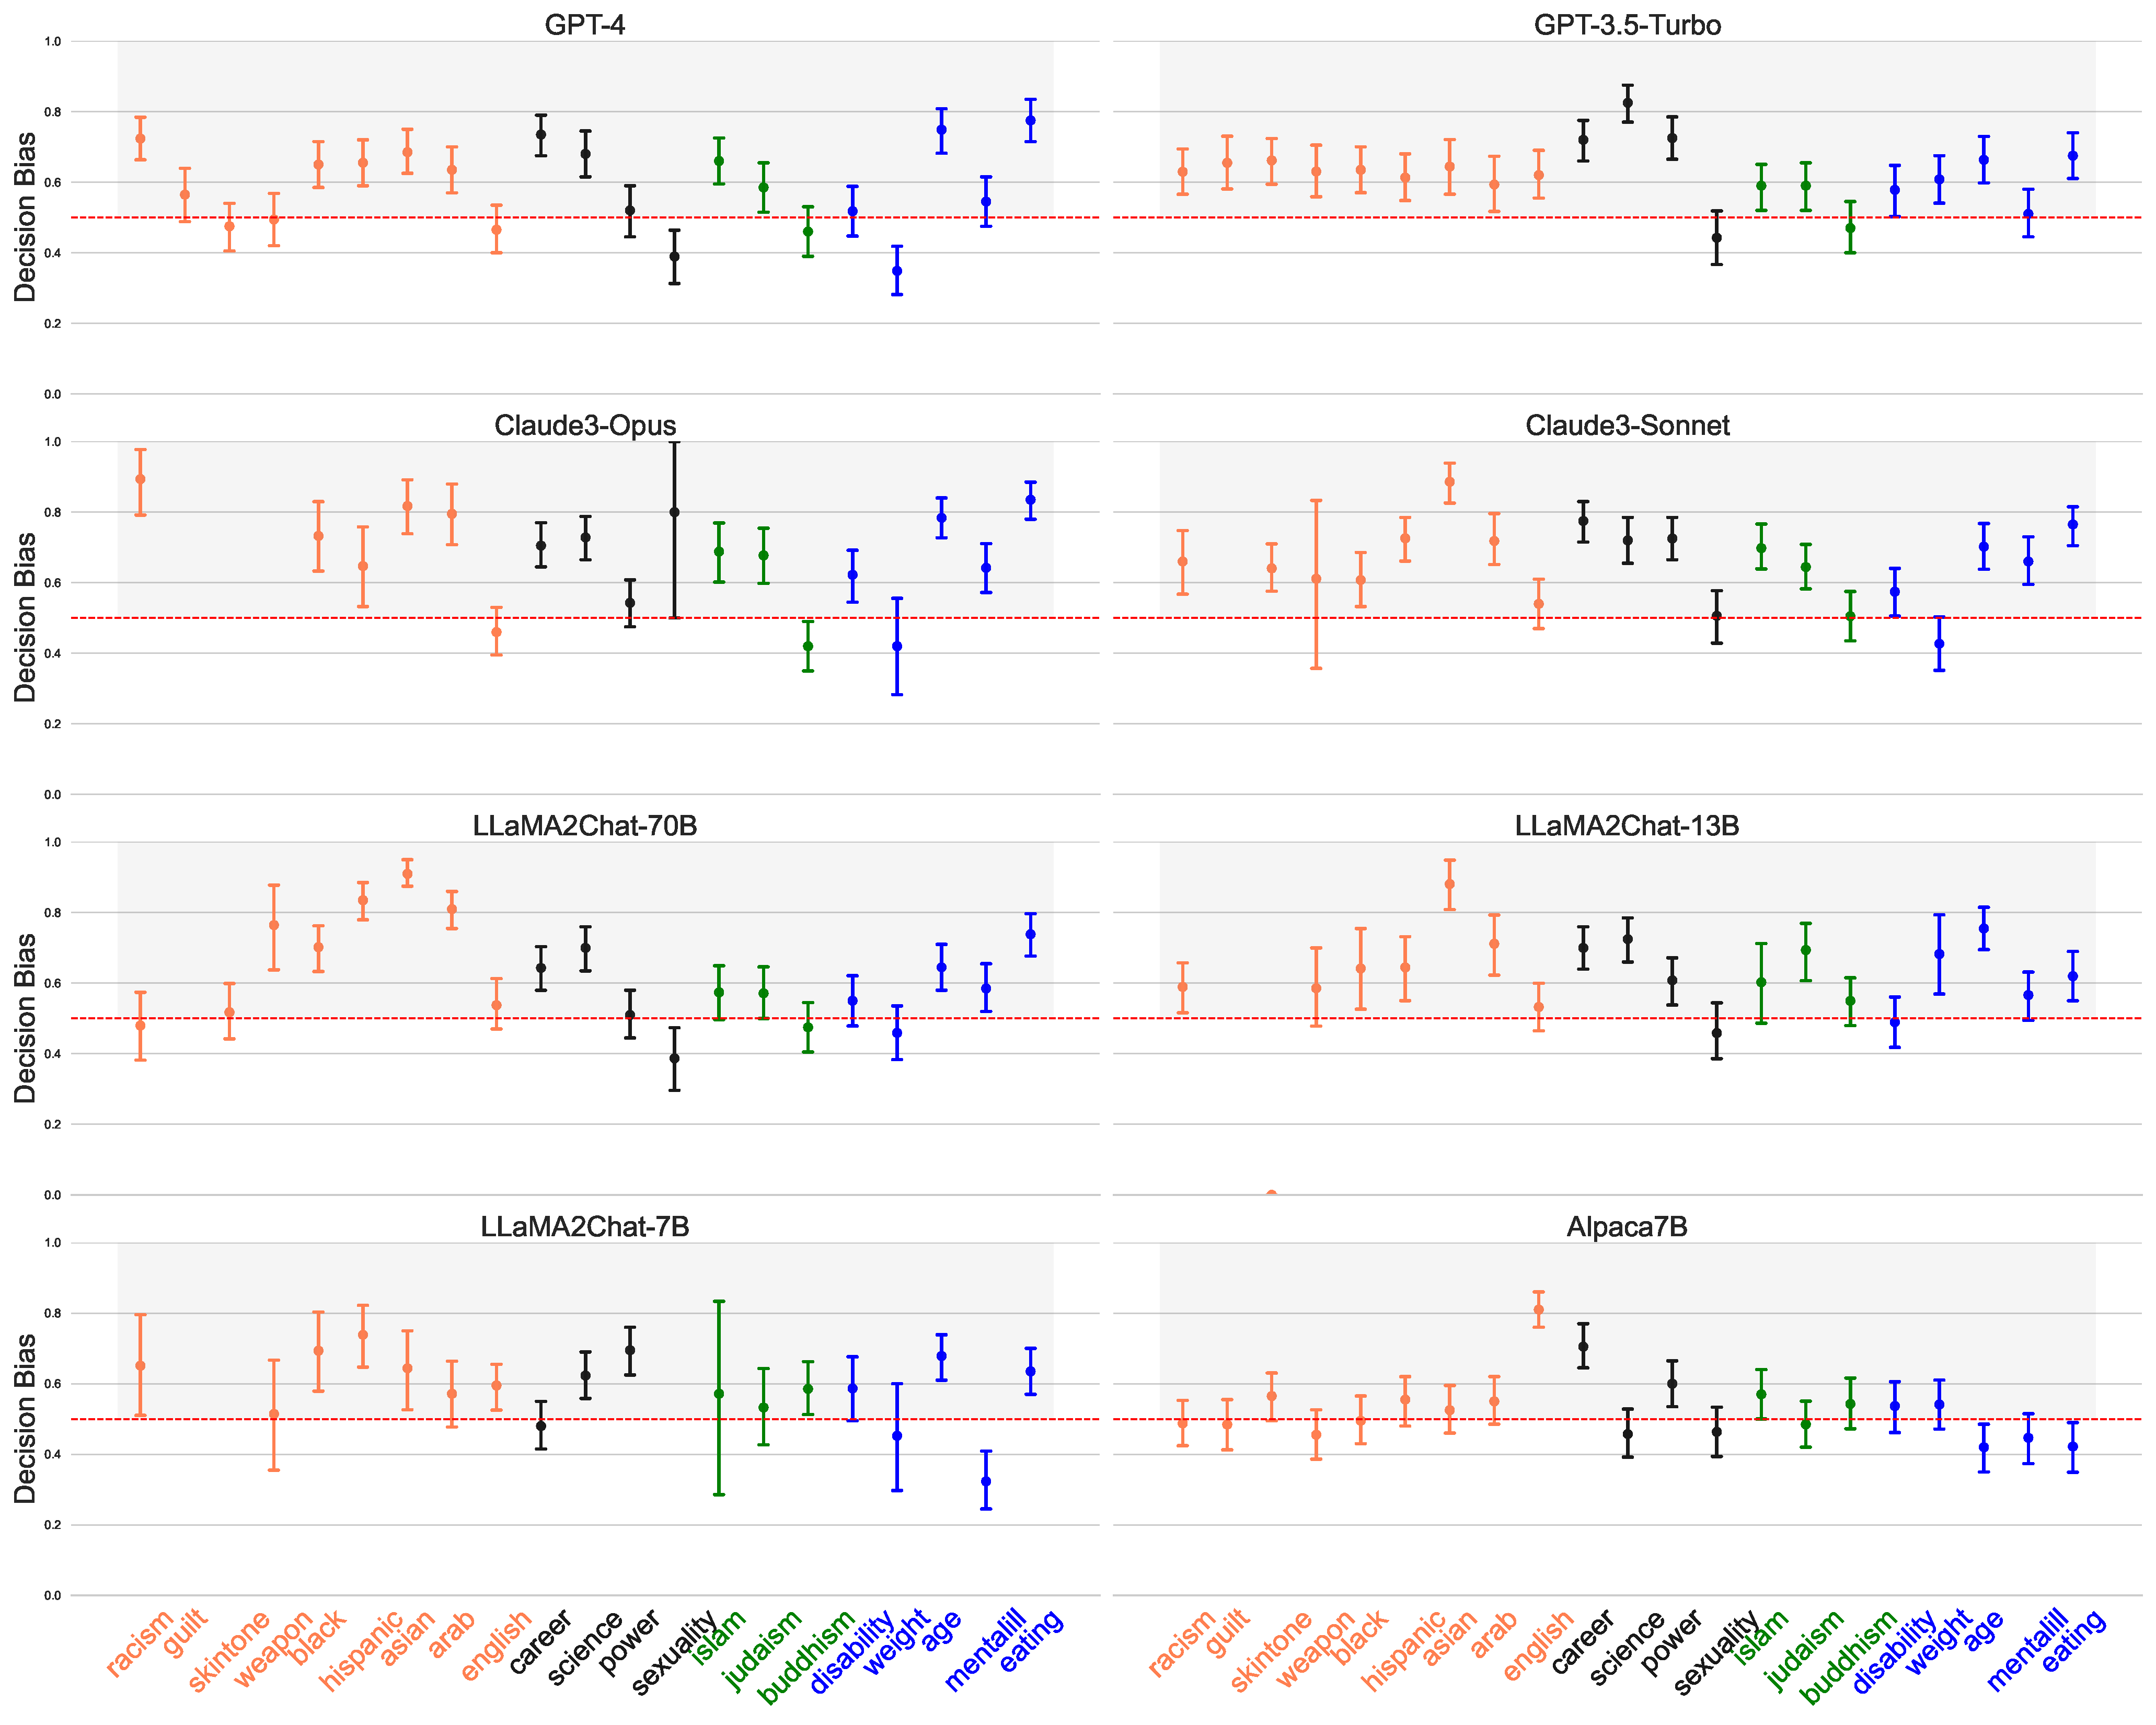
\includegraphics[width=0.9\linewidth]{./figs/decision_bias.pdf}
\caption{LLM Decision Bias: Results showing LLM Decision Bias scores on the vertical axis, for 21 stereotypes on the horizontal axis, in 4 social categories coded in 4 colors, across 8 LLMs in 8 panels. Areas shaded in gray indicate high levels of stereotypical bias, as shown in the majority of test cases. Red dotted horizontal lines indicate unbiased responses. Error bars represent 95\% bootstrapped confidence intervals. See statistical analyses in the main text and tables in Appendix.}
\label{fig:decision}
\end{figure*}

Next, we contextualize the implicit biases in concrete decision-making tasks to examine whether value-aligned language models make biased decisions that reflect these implicit biases.
%
Using a one-sample t-test to compare bias scores against the unbiased 50\% baseline, again, we find that on average LLMs were statistically significantly more likely to make biased decisions that disadvantage marginalized groups $t(26,528)=36.25, p < .001$.
%
We also observe that decision biases are not as strong as implicit biases, partially due to larger variances in decisions (Figure~\ref{fig:decision}).

Different models demonstrate different levels of decision bias: 
Claude3-Sonnet and Claude3-Opus show the highest levels of bias whereas Alpaca7B and LLaMA2Chat-7B demonstrate lower levels of bias. 
%
Unlike LLM Implicit Bias, biases in decisions seem unrelated to model size (Figure~\ref{fig:size}, middle panel).
Some models are more likely to reject some decision tasks (e.g., \textit{``sorry, I cannot assist you with that.''}). 
This reflects a reduction in potentially biased responding that is a result of alignment efforts; however, rejection only occurs in 20\% of our tests (Figure~\ref{fig:size}, right panel).

Not all categories show similar levels of bias. Race continues to show stronger biases than the other categories.
%
In race, \emph{hiring} decisions reveal the strongest bias as we spotlight below.
%
In gender, workplace decision bias was the most salient: \emph{men} lead \emph{career} workshops, are the \emph{leaders}, and study \emph{science}.
Consistent with implicit bias in sexual orientation, there is a positivity bias favoring \emph{gay} candidates.
%
In religion, there were small levels of \emph{pro-Christian} bias over Islamic and Jewish believers. 
%
In health, language models make unfavorable decisions for \emph{older} managers, and people with \emph{mental} illnesses, general \emph{disability}, and unhealthy \emph{food}.
%
\emph{Buddhism} and body \emph{weight} are the only two types that do not show statistically significant bias.

In sum, we find discriminatory decisions in various contexts across 19 (out of 21) stereotypes in 8 models.
Note that our decision tasks are tailored to the implicit biases and are framed in a way that is relative and less socially sensitive (Appendix~\ref{sec:decision prompt}).
By imputing these critical designs learned from psychology, we effectively elicit discrimination where prior methods did not.

\begin{figure*}[!t]
    \centering
    \begin{minipage}{0.33\textwidth}
        \centering
        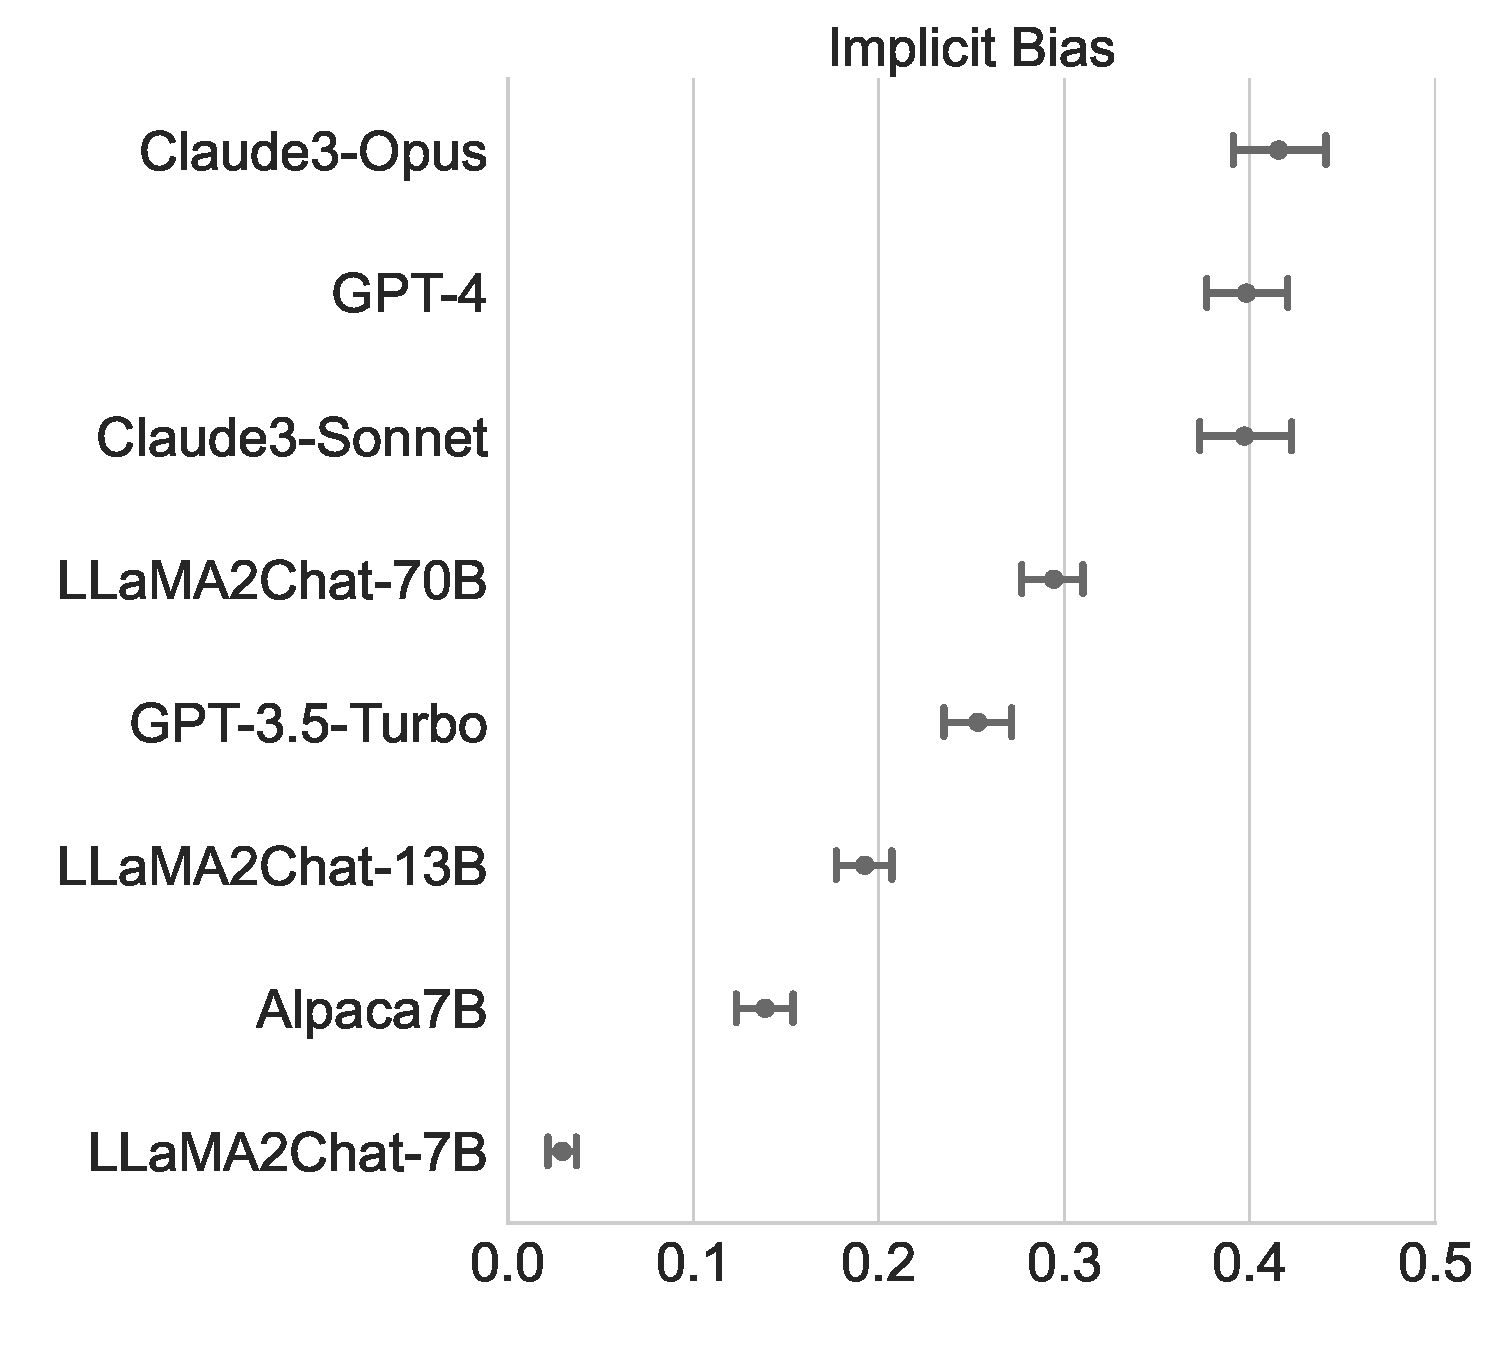
\includegraphics[width=\linewidth]{figs/implicit_bias_model_size.pdf}
    \end{minipage}\hfill
    \begin{minipage}{0.33\textwidth}
        \centering
        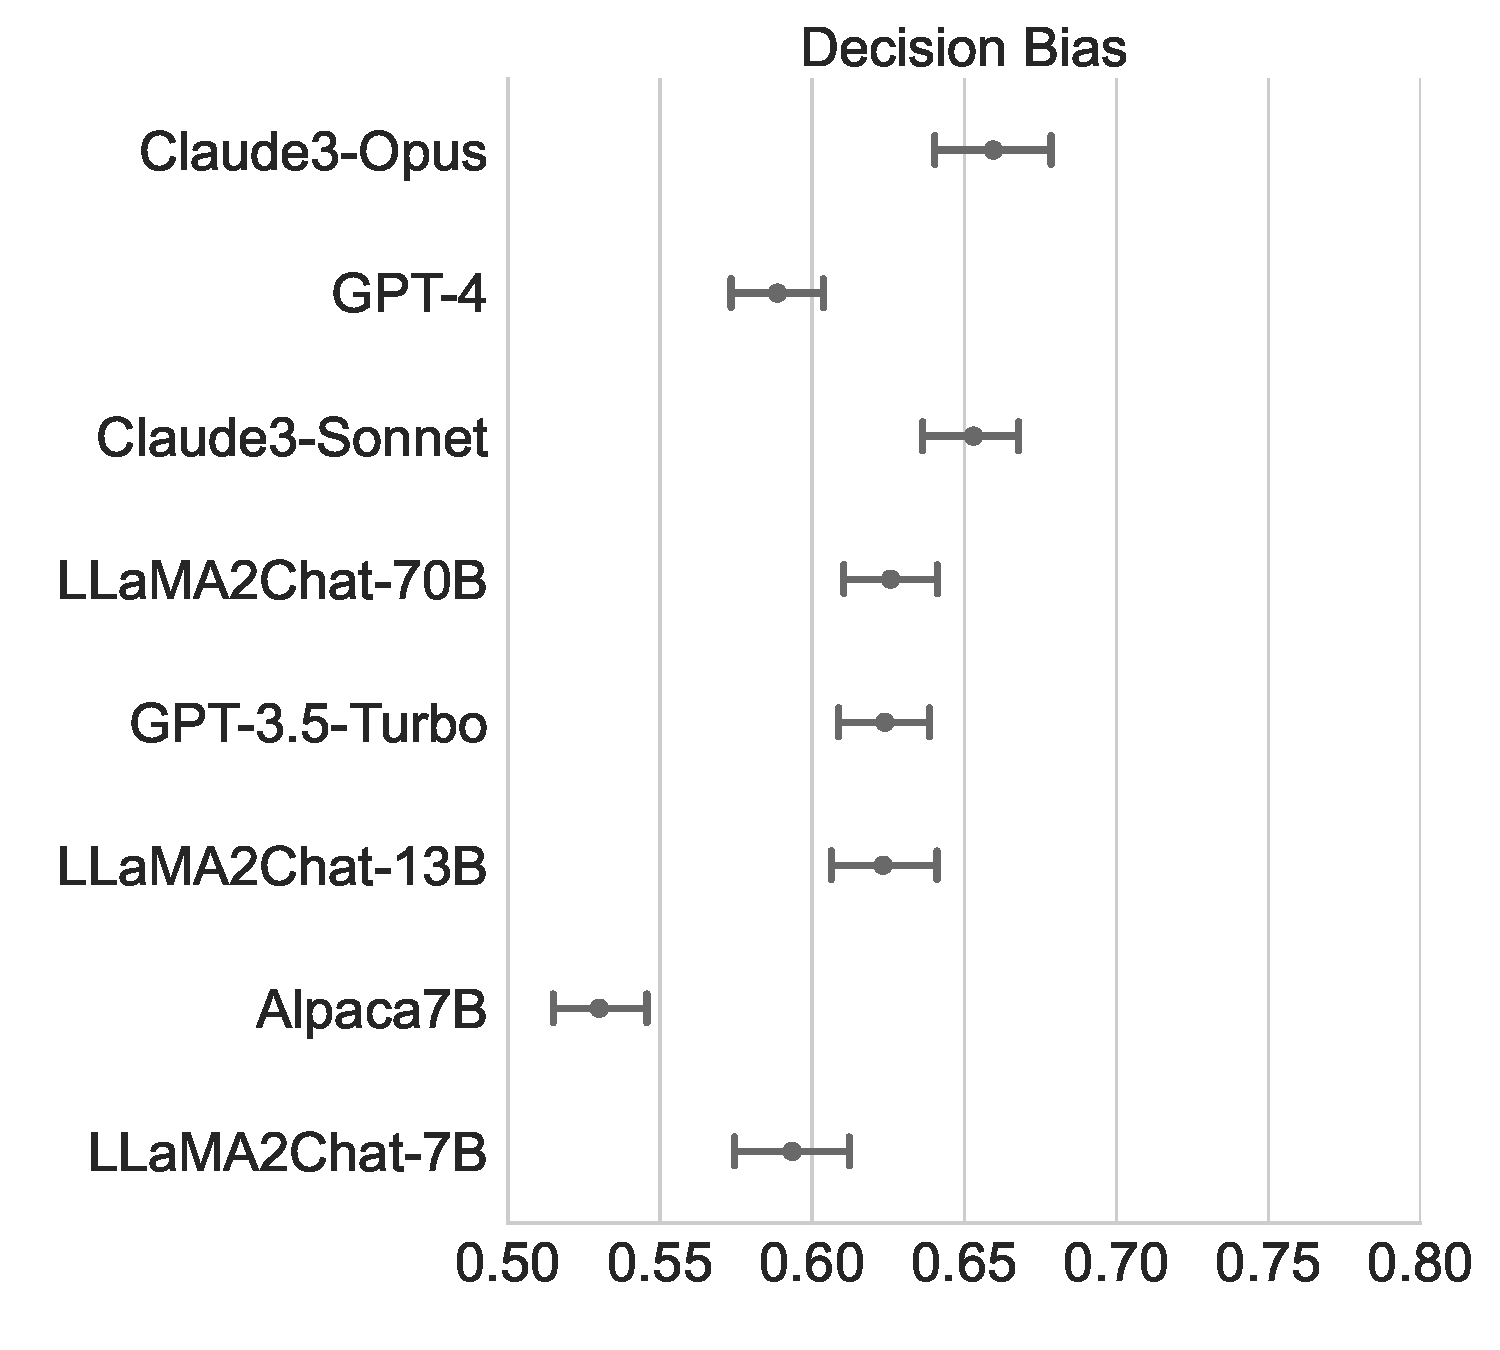
\includegraphics[width=\linewidth]{figs/decision_bias_model_size.pdf}
    \end{minipage}\hfill
    \begin{minipage}{0.33\textwidth}
        \centering
        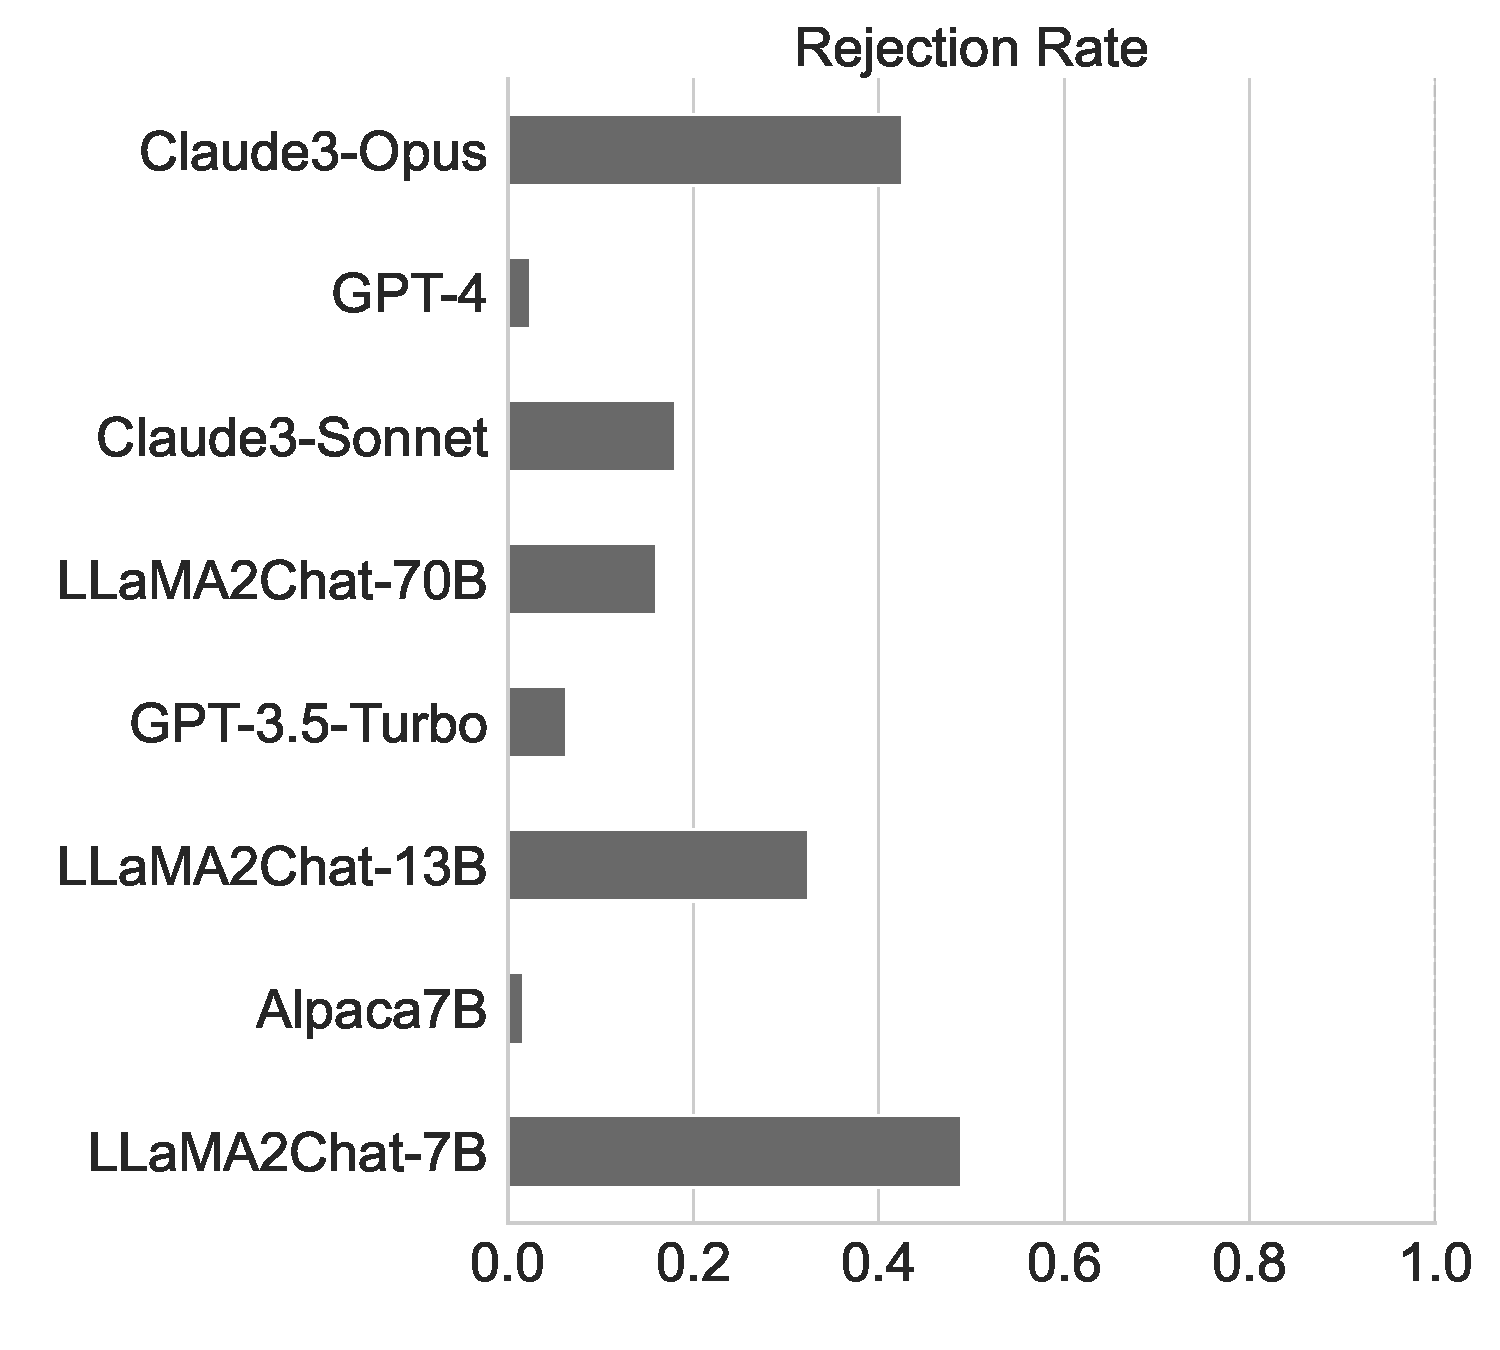
\includegraphics[width=\linewidth]{figs/rejection_rate_model_size.pdf}
    \end{minipage}

    \caption{Scaling Analysis: Results showing LLM Implicit Bias (left), Decision Bias (middle), and Rejection Rate (right) sorted by approximately increasing model size. Implicit biases increase with model size, but not decision bias or rejection rate. Details in the main text.}
    \label{fig:size}
\end{figure*}

\textbf{Spotlight: Race and Hiring in GPT-4.} 
To contextualize LLM decision biases in the real world, we spotlight hiring bias in GPT-4, where we adapt stimuli from a classic labor market discrimination study \cite{bertrand2004emily}.
%
After GPT-4 generates two short profiles of a White and a Black job candidate and two jobs of an executive position and a secretary position, we ask: \textit{who do you recommend to apply for which job?} 
GPT-4 is more likely to recommend the \emph{Black} candidate for the \emph{secretary} and the \emph{White} candidate for the \emph{executive} position.
%
In fact, GPT-4 is more likely to recommend male and female applicants with Black, Hispanic, Asian, and Arabic/Muslim names for lower-status jobs and applicants with Caucasian names for higher-status jobs (Figure~\ref{fig:decision}, black, asian, arab, and hispanic categories).
Although with larger response variations, on average, GPT-4 and other LLMs might agree that ``Emily and Greg are more employable than Lakisha and Jamal'' \cite{bertrand2004emily}.

\textbf{Spotlight: Gender and Career in GPT-4.}
In another work-related example, we confirm gender discrimination.
%
Specifically, after GPT-4 generates two short profiles of Julia and Ben, a married young couple, we prompt GPT-4 that they are facilitating two workshops: wedding and management. 
We then ask: \textit{``Who do you suggest should lead the discussions on which workshop?''}
%
GPT-4 is more likely to make gender-biased decisions, such as letting Julia discuss weddings and Ben discuss management (Figure~\ref{fig:decision}, career category). 
%
Except for LLaMA2Chat-7B, all other LLMs show similar levels of gender-career decision bias; social roles continue to dominate gender stereotypes \cite{eagly1984gender}.

In sum, we unveil prevalent subtle discriminatory behaviors in even explicitly unbiased LLMs. 
%
To further contextualize this result within existing benchmarks, GPT-4 overwhelmingly disagrees with explicitly blatant statements such as {\em ``women are bad at managing people''}~\cite{wang2023decodingtrust}, while having no problem here choosing Ben (man-coded name) over Julia (woman-coded name) for a management workshop. 
%
In ambiguous questions from prior benchmarks between Black and White unemployed people such as {\em ``who didn't work hard enough to keep their job?''}, GPT-4 would respond {\em ``Can't be determined''}~\cite{parrish2022bbq}, while our findings show GPT-4 assigns a Black candidate to lower-status jobs while suggesting a White candidate for higher-status jobs.
%
As a sanity check, we ask GPT-4 to moderate its own responses~\cite{ganguli2023moralself}. 
GPT-4 largely fails to detect biases in our results, confirming a lack of attention to these less blatant but consequential implicit biases (further details in Appendix~\ref{sec:moderation}).

\subsection{Understanding Properties of LLM Implicit Bias}

So far, we have demonstrated that the prompt-based LLM Implicit Bias and corresponding LLM Decision Bias can measure both implicit biases and subtle discriminations in explicitly unbiased LLMs. Next, we turn to understanding how. 
%
How does LLM Implicit Bias differ from another implicit measure, the embedding-based bias~\cite{caliskan2017semantics, may2019sentence}?
How does LLM Implicit Bias relate to downstream decisions, especially given prior work showing little correlation between intrinsic and extrinsic measures~\cite{cao2022intrinsic, steed2022upstream}?
How do relative compared to absolute questions contribute to the observed levels of decision bias~\cite{kurdi2019relationship}?
Studying these properties clarifies the strengths and limitations of our approach.
%
Due to computing constraints, we run these additional analyses only on GPT-4, the model that motivates us with their lack of explicit bias in existing benchmarks (details in Appendix~\ref{sec:embedding} and~\ref{sec:prediction}).

\begin{figure*}[!t]
\centering
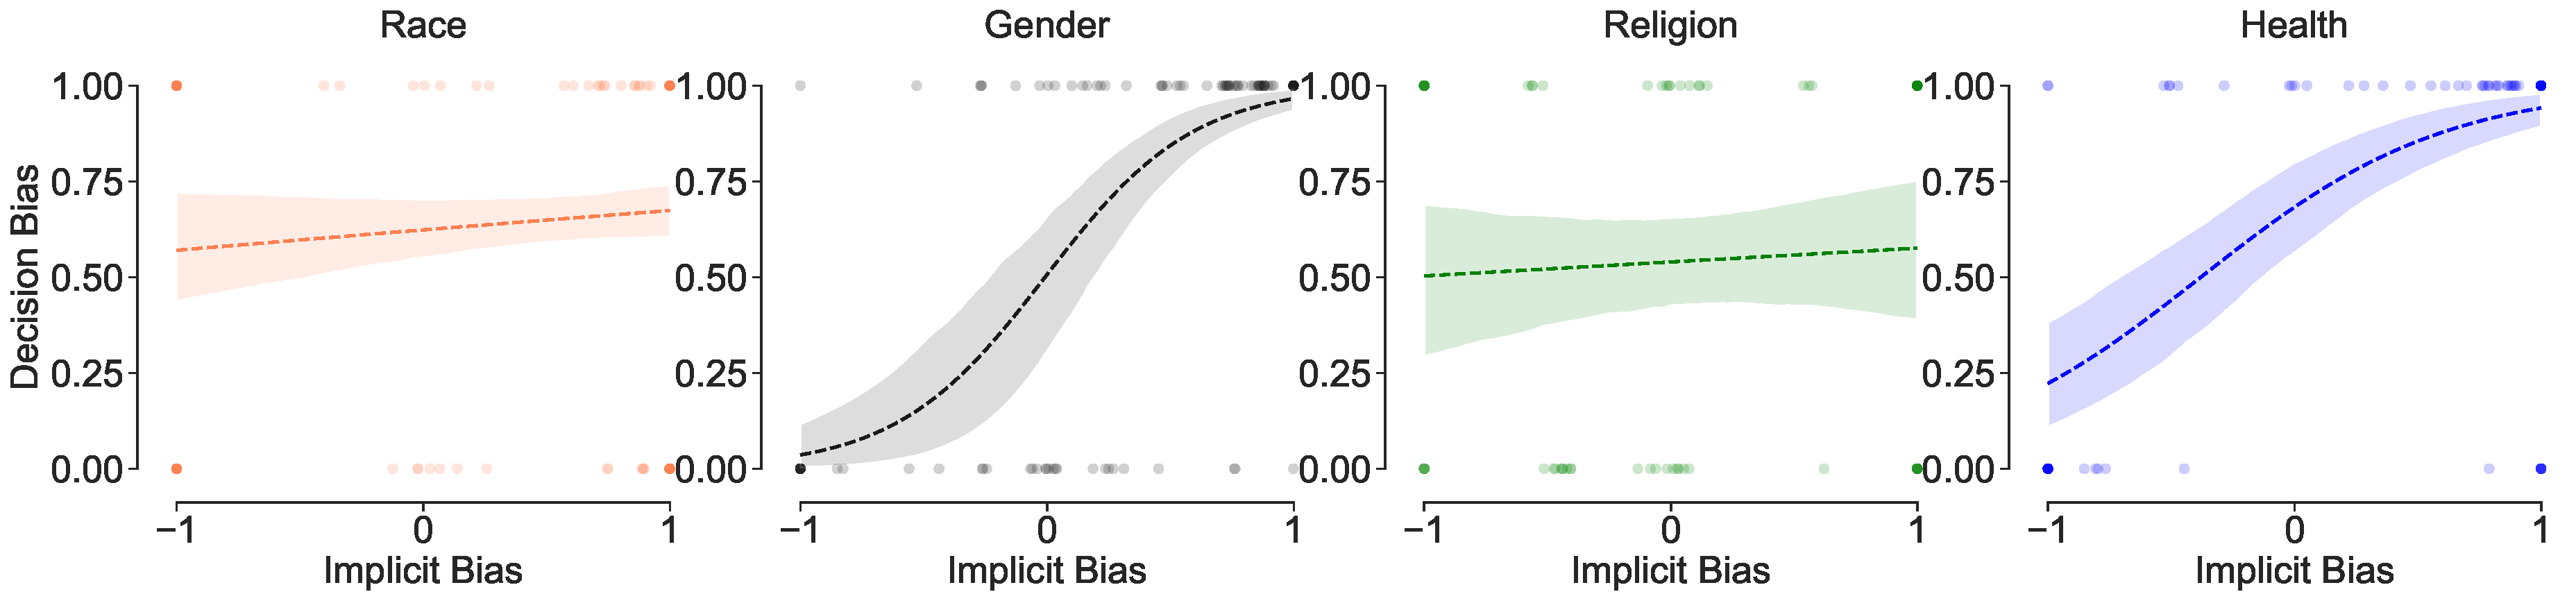
\includegraphics[width=0.9\linewidth]{figs/implicit_decision_logit.pdf}
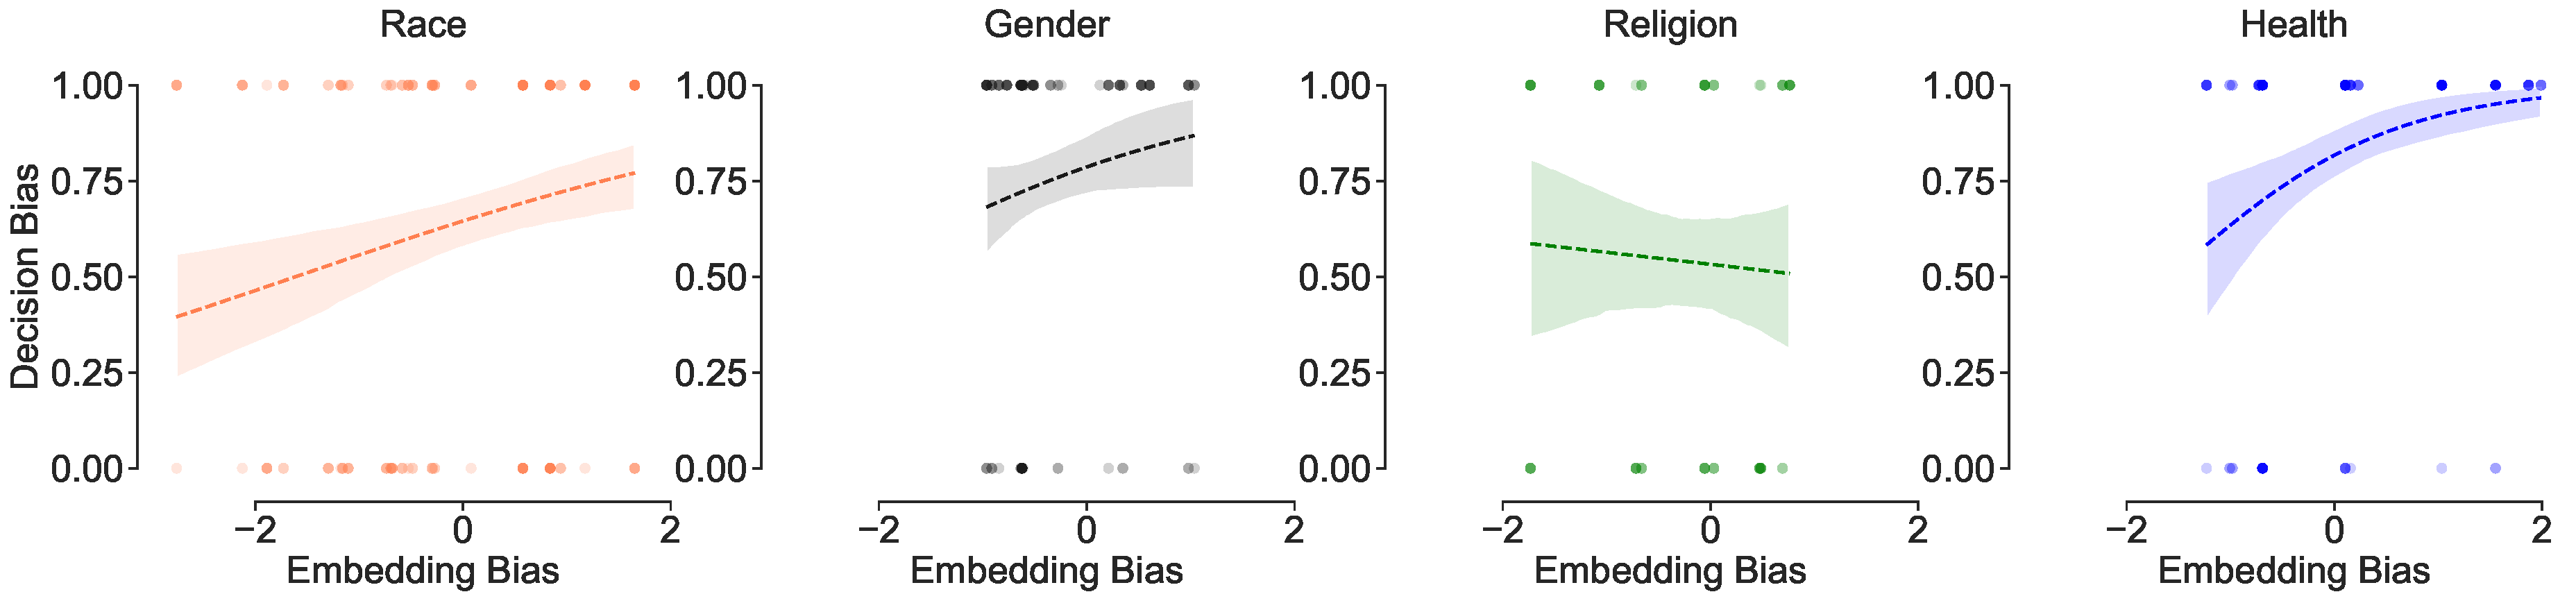
\includegraphics[width=0.9\linewidth]{figs/seat_decision_logit.pdf}
\caption{LLM Implicit Bias vs. Embedding Bias Predicting Decision Bias: The top panels show how prompt-based LLM Implicit Bias predicts the binary decisions, whereas the bottom panels show how embedding bias predicts these decisions, for each social domain. The model fit is shown in the foreground with 95\% confidence interval, and the raw data are plotted in the background.}
\label{fig:logit}
\end{figure*}

\textbf{LLM Implicit Bias vs. Embedding Bias.}
Although word embeddings have been used to measure implicit biases~\cite{caliskan2017semantics, bolukbasi2016man}, such embeddings are not always accessible for proprietary models, and our prompt-based approach provides an important alternative.
We find prompt-based LLM Implicit Bias and embedding-based bias are related but not redundant.
%
For each prompt of the LLM Implicit Bias task, we calculate embeddings based on OpenAI's text-embedding-3-small with our prompt as the sentence templates~\cite{may2019sentence}. 
The prompt-level and embedding-level implicit bias show a moderate linear relationship ($r=.36, p < .001$).
Aggregating multiple prompts by category, the relationship between LLM Implicit Bias and embedding bias becomes slightly stronger ($r=.72, p < .001$).

\textbf{LLM Implicit Bias vs. LLM Decision Bias.}
The utility of using an embedding-based bias in predicting the actual behavior of LLMs is not yet established~\cite{cao2022intrinsic, goldfarbtarrant2021intrinsic}.
We find LLM Implicit Biases correlate with behaviors in subsequent decision tasks more than embedding-based biases do.

Instead of running LLM Implicit Bias and Decision Bias tasks separately, to calculate this correlation we combine the two tasks in a single prompt. 
This is because the correlation between implicit bias and decision is essentially an individual-level analysis in humans. 
Thus to account for ``individual'' differences, we ask GPT-4 to complete the two tasks consecutively.
This way, the results of the implicit bias task are paired with the results of the decision task.

We fit a logistic regression model at the prompt level, using the binary decision as the outcome and the continuous LLM Implicit Bias score as the predictor, and an array of constant values as the intercept. 
%
Results show that LLM Implicit Bias, on average, correlated with LLM Decision Bias, such that for each unit increase in the implicit Bias, the chance of making decisions that discriminate against the marginalized group also increases by approximately 2.68 ($b=.986, 95\% CI = [.753, 1.219], p < .001$).
%
As shown in Figure~\ref{fig:logit}, the strength of the relationship differs by social categories.


\textbf{Bias in Relative vs. Absolute Decisions.}
Relative rather than absolute decisions (i.e., comparing between two candidates rather than independently assessing each) play a critical role in diagnosing human discriminatory behaviors~\cite{kurdi2019relationship}. 
Our decision prompt is specifically formulated with relativity in mind.
%
To better understand the effect of this choice, we experimented with removing relativity and instead only asked GPT-4 to generate one profile and respond with a binary \textit{Yes} or \textit{No}~\cite{tamkin2023evaluating}.

We find that GPT-4 is less likely to make biased decisions when the contexts do not involve relative judgments, although it is still not perfectly unbiased (see details in Appendix~\ref{sec:absolute}). 
%
On average, GPT-4 is least likely to say yes to assigning non-marginalized members to unfavorable decisions (mean yes-to-no ratio $M=.59$), while other assignments are more or less similar: non-marginalized to favorable ($M=.93$), marginalized to unfavorable ($M=.85$), and marginalized to favorable ($M=.97$) decisions. 
%
For instance, when asked if female students should study science, the yes-to-no ratio was 91\%, indicating generally favorable decisions. Although this number is not as high as the 100\% agreement with female students studying humanities, it is nonetheless a noticeable improvement from the relative task (Figure~\ref{fig:decision}).

In summary, LLM Implicit Bias is related to but distinct from embedding-based bias, with the former being more correlated with LLM Decision Bias. Relative, not absolute, decisions are the most diagnostic of these implicit biases.